\section{Post-review experiments}
\label{sec:extensionresults}
\subsection{Equal acquisition budgets expose a different FN/FP compromise}
Table~\ref{tab:tonextension} reports the new TON runs with independent seed/block randomization. The spline head with CAL64 attains 89.46\% recall and 19.78\% FPR. A frozen spline detector using all acquired labels through CAL256 attains higher recall, 92.38\%, with 48.14\% FPR. The head therefore trades 2.92 recall points for a 28.36-point FPR reduction; its BA gain is 12.72 points. In counts, the mean difference is $+94{,}549.4$ FN and $-87{,}825.2$ FP. All five seeds incur more FN and fewer FP. This is a consistent trade-off, not joint error dominance.

\begin{table}[tb]
\centering\fontsize{8.8}{10.5}\selectfont\setlength{\tabcolsep}{4pt}
\caption{Post-review TON D results, five seeds: mean $\pm$ sample SD. Recall, FPR, and BA are percentages. The last column is macro block AUROC. All methods receive the same acquired labels; their use of those labels and model memory differs as specified in Table~\ref{tab:extensiondesign}.}
\label{tab:tonextension}
\begin{tabular}{lrrrr}
\toprule
Controller & Recall & FPR & BA & AUROC \\
\midrule
\tablerows{tables/ton_extension_rows.tex}
\bottomrule
\end{tabular}
\end{table}

The stronger threshold-only baseline changes the interpretation of the residual gain. Against CAL256, the spline head adds 75,144.6 FN and removes 79,459.4 FP in the seen stratum. On unseen vectors it adds 19,404.8 FN and removes 8,365.8 FP on average; two seeds improve both error counts there. Thus 90.5\% of the FP reduction is still concentrated on previously observed vectors, but the unseen recall improvement observed against the original CAL64 control is no longer a general finding. Figure~\ref{fig:newstrata} shows the paired rate differences. The control used to define ``additional benefit'' is consequential.

\begin{figure}[tb]
\centering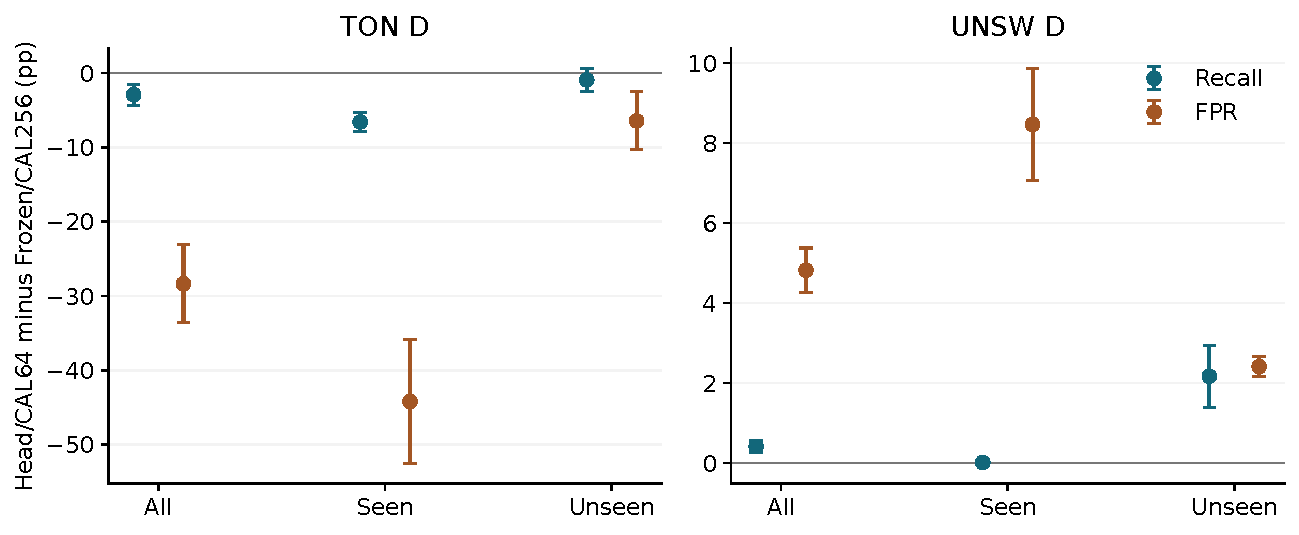
\includegraphics[width=\linewidth]{figures/fig6_stratum_effects.pdf}
\caption{Spline FIT192/CAL64 minus Frozen/CAL256, by reporting stratum. Points are paired seed means; bars are sample SDs. Positive recall differences and negative FPR differences favor the head. When both rates move in the same direction, the policy trades recall against false alarms.}
\label{fig:newstrata}
\end{figure}

The linear head reaches 84.80\% BA, close to the spline head's 84.84\%, with 88.96\% recall and 19.36\% FPR. Its frozen/CAL256 control reaches 87.20\% recall and 43.10\% FPR. The allocation of gain between recall and false alarms is therefore model-dependent even on the same requested labels.

The standard stream learner changes the picture further. ARF at its natural threshold 0.5 reaches 97.98\% recall, 19.03\% FPR and 89.47\% BA; ARF/CAL256 reaches 96.41\%, 15.62\% and 90.39\%, respectively. Its own frozen/CAL256 control reaches only 67.87\% BA. ARF/CAL256 reduces both error counts relative to that control in every TON seed. This is substantial learning benefit beyond threshold adaptation for the tested forest, under its more permissive model-memory and calibration-reuse contract. It also prevents the spline-head findings from being generalized to all adaptive IDS learners.

\subsection{Which proposed mechanisms survive direct controls?}
\begin{table}[tb]
\centering\small\setlength{\tabcolsep}{4pt}
\caption{Spline controls in the new campaign, five seeds. Rates are mean $\pm$ sample SD in percent. Independent CAL64 equals the matched CAL64 outcomes in these runs.}
\label{tab:ablations}
\begin{tabular}{llrrr}
\toprule
Dataset & Controller & Recall & FPR & BA \\
\midrule
\tablerows{tables/ablation_rows.tex}
\bottomrule
\end{tabular}
\end{table}

Independently updating CAL64 produces the same decisions as the matched-gate control in both datasets' main runs. Removing the head gate alone therefore does not explain the large original FP contrast. Both versions still require enough recent calibration observations; on development C, the recorded starvation was caused by missing normal CAL labels, so this change alone would not remove that eligibility condition.

The intercept-only/CAL64 trace exactly matches frozen/CAL64 confusion counts in every new spline and linear run, as expected from threshold-shift invariance. Its fixed-B trace can move recall markedly, but that demonstrates an operating-point change rather than new discrimination. Prior-centred regularization also does not supply a uniform remedy. For the spline model, it yields 84.42\% BA on TON versus 84.84\% for the zero-centred refit, and 93.72\% on UNSW versus 93.22\%. The regularization centre affects the result, but the tested alternative does not establish a generally preferable update rule (Table~\ref{tab:ablations}).

\subsection{A separate capture reverses the aggregate preference}
\begin{table}[tb]
\centering\fontsize{8.8}{10.5}\selectfont\setlength{\tabcolsep}{4pt}
\caption{Separate chronological UNSW-NB15 D evaluation, five seeds, with the same reporting conventions as Table~\ref{tab:tonextension}. Each model is trained anew on that dataset's A partition.}
\label{tab:unswextension}
\begin{tabular}{lrrrr}
\toprule
Controller & Recall & FPR & BA & AUROC \\
\midrule
\tablerows{tables/unsw_extension_rows.tex}
\bottomrule
\end{tabular}
\end{table}

On UNSW-NB15, the frozen spline model at its initial B threshold already reaches 94.53\% recall, 1.95\% FPR, and 96.29\% BA (Table~\ref{tab:unswextension}). Recent CAL256 selection raises recall to 96.37\%, but raises FPR to 5.53\%. Adding the head gives 96.79\% recall and 10.36\% FPR, reducing BA to 93.22\%. Against CAL256, the head removes 885.0 FN while adding 38,754.6 FP; every seed has that same directional trade-off. On unseen vectors its mean recall gain is 2.17 points and its FPR increase is 2.41 points, leaving a mean BA difference of $-0.12$ points.

The linear model also illustrates why the baseline matters: its head/CAL64 BA is 91.39\%, below frozen/CAL256 at 91.86\%, although it exceeds frozen/CAL64 at 89.75\%. A small calibration memory can make adaptation appear more beneficial than it is against a controller using all acquired labels. The second capture therefore supports the need for decomposition, while contradicting a universal claim that the specific adaptive head improves detection.

ARF/CAL256 reaches 96.49\% recall, 4.77\% FPR and 95.86\% BA on UNSW. Its BA exceeds its own frozen/CAL256 baseline in every seed; the latter is highly variable across initial fits and averages 60.74\% BA. Nevertheless, none of these paired UNSW seeds improves both FN and FP at once. Even for a strong stream learner, mean error reductions and consistent BA gains must be distinguished from per-seed joint dominance. The frozen spline/B detector retains the highest mean BA among the displayed default policies on this capture, at 96.29\%.

\subsection{Causally selected operating points and label sensitivity}
\begin{figure}[tb]
\centering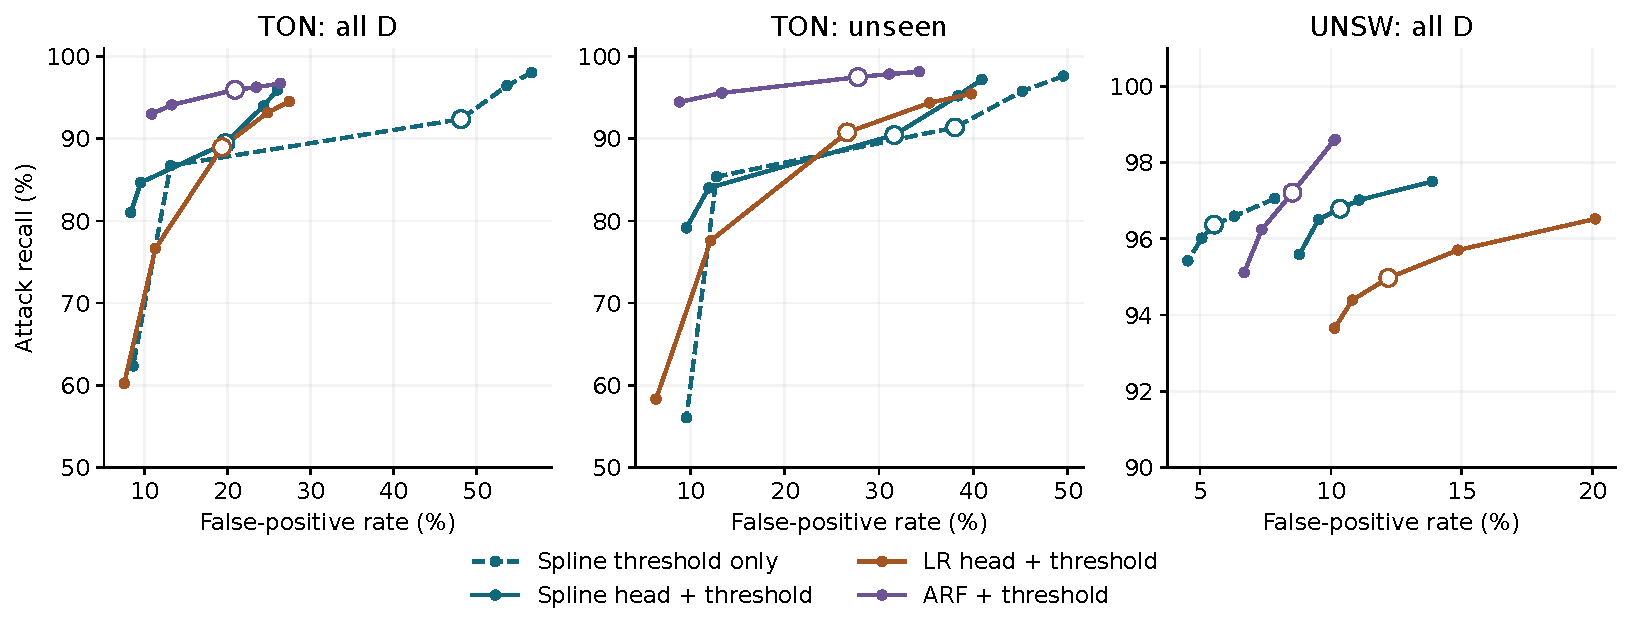
\includegraphics[width=\linewidth]{figures/fig5_cost_tradeoffs.pdf}
\caption{Operating points generated by five pre-specified rate-cost weights, each threshold fitted only to past available labels. Connected points belong to one controller; hollow markers denote $\lambda=1$. Vertical ranges differ to expose the observed variation. The display compares realized future errors, rather than an oracle frontier optimized on evaluation labels. Means are over five paired seeds; individual results are supplied in the accompanying CSV tables.}
\label{fig:tradeoffs}
\end{figure}

Figure~\ref{fig:tradeoffs} expresses the practical question as a family of explicit error compromises. It prevents the BA optimum from being mistaken for a unique preferred detector. The error-cost weight, available labels, and score function jointly determine which future operating points are reached. A preferred point consequently requires an application-specific alarm burden and missed-attack cost.

Delay and label scarcity materially change those points (Table~\ref{tab:sensitivity}). For the spline head on TON, BA decreases from 85.90\% at delay zero to 84.84\%, 82.87\%, and 80.07\% at delays one, five, and twenty. At a 0.1\% budget and delay one, recall falls to 32.13\% and BA to 57.49\%; the frozen/CAL256 controller retains 86.22\% recall and 79.48\% BA. This is a consequence of the tested finite-memory and eligibility policy under fewer labels, not evidence that every adaptive learner has the same sensitivity.

\begin{table}[tb]
\centering\fontsize{8.5}{10}\selectfont\setlength{\tabcolsep}{3.4pt}
\caption{TON spline sensitivity, five seeds. The default budget is 1\%; only the last pair uses 0.1\%. Rates are percentages. Updates count eligible decisions, including the final decision without a subsequent evaluated block.}
\label{tab:sensitivity}
\begin{tabular}{llrrrr}
\toprule
Condition & Controller & Recall & FPR & BA & Updates \\
\midrule
\tablerows{tables/sensitivity_rows.tex}
\bottomrule
\end{tabular}
\end{table}

The nominal 1\% budget corresponds to 35,499 queried labels during 62.77 observed hours of TON D, approximately 566 labels per hour. UNSW D requires 10,160 labels during 7.89 hours, approximately 1,288 per hour. These volumes describe an annotation service assumption rather than a single analyst's feasible workload. Measured query-to-arrival times have medians near 3.50 minutes on TON and 6.45 minutes on UNSW; their approximate 95th percentiles are 54.6 and 12.5 minutes, respectively. The exact per-seed distributions are provided with the results. A one-block delay is therefore neither a constant number of seconds nor a guarantee of realistic incident-confirmation latency.

\subsection{Ranking summaries, attack families, and computational accounting}
Pooled fixed-score AUROC and two block summaries are reported in Table~\ref{tab:aucsupp}; per-family attack recall appears in Table~\ref{tab:attacksupp}. These quantities answer different questions. In particular, macro block AUROC gives a block with few normal observations the same weight as a block with many. Normal-count weighting is a sensitivity summary, while pooling the fixed score also compares observations across time. Neither is substituted silently for the original statistic.

All additional runs record initial fitting, initial B scoring, cached feature/score preparation, replay components, and serialization sizes. The initial artifact contains the base model and transform; the final size counts only the base model object. Both exclude label memories, the pending queue, inference caches and separately held linear-head vectors, and neither measures total controller RAM. The extension reuses immutable representations and identical-vector predictions within a fixed forest state to accelerate the offline study. Consequently, cached replay time alone is not an end-to-end inference benchmark. The complete cost ledger reports preparation separately, and the forest's persistent tree state is not described as satisfying a 256-example total-memory bound. No embedded latency or energy claim follows from these measurements.
